\documentclass{article}

\usepackage[english]{babel}

\usepackage[letterpaper,top=2cm,bottom=2cm,left=3cm,right=3cm,marginparwidth=1.75cm]{geometry}

% Useful packages
\usepackage{amsmath}
\usepackage{amssymb}
\usepackage{xcolor}
\usepackage{graphicx}
\usepackage{mathtools}
\usepackage{framed}
\usepackage{tikz}
\usepackage[colorlinks=true, allcolors=blue]{hyperref}
\usepackage{xcolor}
\usepackage{colortbl}
\usepackage{booktabs}
\usepackage{tikz}
\usepackage{tcolorbox}
\usepackage{algorithm}
\usepackage{algpseudocode}
\usepackage{amsthm}
\usetikzlibrary{positioning, arrows.meta}

\theoremstyle{definition}
\newtheorem{exmp}{Example}[section]

\definecolor{sigblue}{RGB}{214,228,247}
\definecolor{siggreen}{RGB}{208,235,203}
\definecolor{sigyellow}{RGB}{255,245,200}

\newcommand{\Fp}{\mathbb F_p}
\newcommand{\Fq}{\mathbb F_q}
\newcommand{\offdest}{\text{off}_{\text{dest}}}
\newcommand{\offopzero}{\text{off}_{\text{op0}}}
\newcommand{\offopone}{\text{off}_{\text{op1}}}
\newcommand*{\logeq}{\ratio\Leftrightarrow}

\algnewcommand\algorithmicpublicinput{\textbf{Public input:}}
\algnewcommand\publicinput{\item[\algorithmicpublicinput]}

\algnewcommand\algorithmicprivateinput{\textbf{Private input:}}
\algnewcommand\privateinput{\item[\algorithmicprivateinput]}

\newtheorem{lemma}{Lemma}

\title{Minimal zkVM for Lean Ethereum (draft 0.6.0)}
\date{}
\begin{document}

\maketitle

\section{What is the goal of this zkVM?}

Replacing the BLS signature scheme with a Post-Quantum alternative. One approach is to use stateful hash-based signatures, XMSS, as explained in \cite{ethereum_signatures}, \cite{top_hypercube} and \cite{LeanSig}, and to use a hash-based SNARK to handle aggregation.
A candidate hash function is Poseidon2 \cite{poseidon2}.

We want to be able to:

\begin{itemize}
    \item \textbf{Aggregate} XMSS signatures
    \item \textbf{Merge} those aggregate signatures
\end{itemize}

The latter involves recursively verifying a SNARK. Both tasks mainly require to prove a lot of hashes. A minimal zkVM (inspired by Cairo \cite{cairo}) is useful as glue to handle all the logic.

Aggregate / Merge can be unified in a single program, which is the only one the zkVM has to prove (see \ref{fig1} for a visual interpretation):

\begin{algorithm}
\caption{AggregateMerge}
\begin{algorithmic}[1]
\publicinput \textbf{pub\_keys} (of size $n$), \textbf{bitfield} ($k$ ones, $n-k$ zeros), \textbf{msg} (the encoding of the signed message)
\privateinput $s > 0$, \textbf{sub\_bitfields} (of size $s$), \textbf{aggregate\_proofs} (of size $s - 1$), \textbf{signatures}


\Comment{Bitfield consistency}

\State Check: \textbf{bitfield} $= \bigcup_{i=0}^{s-1}$
\textbf{sub\_bitfields}[i]


\State \Comment{Verify the first $s-1$ sub\_bitfields using aggregate\_proofs:}

\For{$i \gets 0$ to $s-2$}
    \State inner\_public\_input $\gets$ (\textbf{pub\_keys}, \textbf{sub\_bitfields}[i], \textbf{msg})
    \State \textit{snark\_verify}("AggregateMerge", inner\_public\_input, \textbf{aggregate\_proofs}[i])
    % \State  \Comment{\textbf{snark\_verify}(program, public input, proof)}
\EndFor

\State \Comment{Verify the last sub\_bitfields using signatures}

\State $k \gets 0$
\For{$i \gets 0$ to $n-1$}
    \If{\textbf{sub\_bitfields}[s-1][i] = 1}
       \State \textit{signature\_verify}(\textbf{msg}, \textbf{pub\_keys}[i], \textbf{signatures}[k])
       \State $k \gets k + 1$
    \EndIf
\EndFor

\end{algorithmic}
\end{algorithm}



\begin{figure}[h]
\label{fig1}
\caption{AggregateMerge visualized.}
\centering
\includegraphics[scale=0.6]{images/AggMerge.png}
\end{figure}


\section{VM specification}
\subsection{Field}

\fbox{KoalaBear prime: $p = 2^{31} - 2^{24} + 1$}

\vspace{3mm}

Advantages:
\begin{itemize}
    \item small field $\xrightarrow{}$ less Poseidon rounds
    \item $x \xrightarrow{} x^3$ is an automorphism of $\Fp^*$, meaning efficient S-box for Poseidon2 (in BabyBear, it's degree $7$)
    \item $< 2^{31}$ $\xrightarrow{}$ the sum of 2 field elements can be stored in an u32
\end{itemize}

The small 2-addicity (24) is not a limiting factor in WHIR, thanks to the use of an interleaved Reed Solomon code.

% For instance, in a degree 8 extension, with rate = $1/2$, FRI/WHIR can commit to a polynomial of degree $2^{26}$ (FFT on a domain of size $2^{27}$), which is to equivalent to $2^{29}$ KoalaBear elements after RingSwitching \cite{fri_binius} $\approx 2 $ GiB of data (enough to prove the validity of $2$ million Poseidon2).


\vspace{3mm}

\fbox{Extension field: of degree 5} : enables 128 bits of security in WHIR, with the Johnson bound, thanks to the latest result of \cite{proximity_gaps_rs_codes_2}.

\subsection{Memory}

\begin{itemize}
    \item Read-Only Memory
    \item Word = KoalaBear field element
    \item Memory size: $M = 2^m$ with $16 \leq m \leq 29$ ($m$ depends on the execution and is communicated at the beginning of the proof).
    \item The first $M' = 2^{m'}$ memory cells hold the "public input", on which both prover and verifier must agree.
    This enables to pass the arguments that the leanISA program receives as input (in our case: message to sign and XMSS public keys).
\end{itemize}

% \begin{figure}[h]
% \caption{Memory structure}
% \centering
% \label{memory}
% \includegraphics[scale=0.7]{images/memory.png}
% \end{figure}

\subsection{Registers}

% As in Cairo:
\begin{itemize}
    \item \fbox{pc: program counter}
    % \item \textbf{ap}: allocation pointer = Points to the first untouched memory cell
    \item \fbox{fp: frame pointer} : points to the start of the current stack
\end{itemize}


\textbf{Difference with Cairo: no "ap" register} (allocation pointer).


\subsection{Instruction Set Architecture}

Notations:
\begin{itemize}
    \item $\alpha$, $\beta$ and $\gamma$ represent parameters of the instructions (immediate value operands)
    \item $\textbf{m}[i]$ represents the value of the memory at index $i \in \Fp$, with $i < M$ ($M$: memory size). Any out-of-bound memory access ($i \geq M$) is invalid.
    \item $\begin{cases} A \\ B \end{cases}$ When using the instruction, either $A$ or $B$ can be used, but not both simultaneously.
\end{itemize}


\subsubsection{ADD / MUL}

$a + c = b$ or $a \cdot c = b$ with: 

\begin{align*}
a &= 
\begin{cases}
\alpha \\
\textbf{m}[\text{fp} + \alpha]
\end{cases}
&
b &= 
\begin{cases}
\beta \\
\textbf{m}[\text{fp} + \beta]
\end{cases}
&
c &= 
\begin{cases}
\text{fp} \\
\textbf{m}[\text{fp} + \gamma]
\end{cases}
\end{align*}


\subsubsection{DEREF}

$$
\textbf{m}[\textbf{m}[\text{fp} + \alpha] + \beta] = 
\begin{cases}
& \gamma \\
& \textbf{m}[\text{fp} + \gamma]   \\
& \text{fp}  

\end{cases}
$$

\subsubsection{JUMP (Conditional)}

\begin{align*}
\text{condition} &= 
\begin{cases}
\alpha \\
\textbf{m}[\text{fp} + \alpha]
\end{cases} \in \{0, 1\}
&
\text{dest} &= 
\begin{cases}
\beta \\
\textbf{m}[\text{fp} + \beta]
\end{cases}
&
\text{updated\_fp} &=
\begin{cases}
\text{fp} \\
\textbf{m}[\text{fp} + \gamma]
\end{cases}
\end{align*}

$$
\text{next(pc)} =
\begin{cases}
\text{dest} & \text{if condition} = 1 \\
\text{pc} + 1 & \text{if condition} = 0
\end{cases}
\qquad
\text{next(fp)} =
\begin{cases}
\text{updated\_fp} & \text{if condition} = 1 \\
\text{fp} & \text{if condition} = 0
\end{cases}
$$

\subsubsection{2 Precompiles}



\begin{enumerate}
    \item \textbf{POSEIDON}: Poseidon2 permutation over 16 field elements.
    \item \textbf{DOT\_PRODUCT}: Computes a dot product between either:
    \begin{itemize}
        \item two slices of extension field elements
        \item one slice of base field elements, and one slice of extension field elements
    \end{itemize}
\end{enumerate}


\subsection{ISA programming}

\subsubsection{Functions}

\begin{enumerate}
    \item Each function has a deterministic memory footprint: the length of the continuous frame in memory that is allocated for each of the its calls.
    \item At runtime, each time we call our function, we receive via a memory cell a hint pointing to a free range of memory. We then store the current values of pc / fp at the start of this newly allocated frame, alongside the function's arguments, we can then jump, to enter the function bytecode, and modify fp with the hinted value. The intuition here is that the verifier does not care where the new memory frame will be placed (we use a read-only memory, so we cannot overwrite previous frames). In practice, the prover that runs the program would need to keep the value of the allocation pointer "ap", in order to adequately allocate new memory frames, but there is no need to keep track of it from the versifier's perspective.
\end{enumerate}


\begin{figure}[h]
\caption{Memory layout of a function call}
\centering
\includegraphics[scale=0.4]{images/memory_layout.png}
\end{figure}

\subsubsection{Loops}\label{loops}

We suggest to unroll loops when the number of iterations is low, and known at compile time.
The remaining loops are transformed into recursive functions (by the leanISA compiler).

\subsubsection{Range checks}

\fbox{It's possible to check that a given memory cell is smaller than some value $t$ (for $t \leq 2^{16})$ in 3 cycles.}

We denote by \textbf{m}[fp + $x$] the memory cell for which we want to ensure \textbf{m}[fp + $x$] $< t$.
We also denote by \textbf{m}[fp + $i$], \textbf{m}[fp + $j$] and \textbf{m}[fp + $k$] 3 auxiliary memory cells (that have not been used yet).
\begin{enumerate}
    \item \textbf{m}[\textbf{m}[fp + $x$]] = \textbf{m}[fp + $i$] (using DEREF, this ensures \textbf{m}[fp + $x$] $ < M$, the memory size)
    \item \textbf{m}[\textbf{m}[fp + $x$]] + \textbf{m}[fp + $j$] = (t-1) (using ADD)
        \item \textbf{m}[\textbf{m}[fp + $j$]] = \textbf{m}[fp + $k$] (using DEREF, this ensures $t - 1 - $ \textbf{m}[fp + $x$] $ < M$)
\end{enumerate}

Given $t \leq 2^{16} \leq M$, \textbf{m}[fp + $x$] $ < M$, $t - 1 - $ \textbf{m}[fp + $x$] $< M$, and $M \leq 2^{29} < p / 2$, we have: \textbf{m}[fp + $x$] $ < t$.

Note: From the point of view of the prover running the program, some hints are necessary (filling the values of \textbf{m}[fp + $i$] and \textbf{m}[fp + $k$] must be done at end of execution).

This idea was pointed out by D. Khovratovich, and is an unplanned use of the DEREF instruction.

\begin{exmp}
	Let's say we want to write a function with 2 arguments $x = \textbf{m}$[fp + 2] and $y = \textbf{m}$[fp + 3] ($\textbf{m}$[fp + 0] and $\textbf{m}$[fp + 1] are used, by convention, to store the caller's pc and fp, to return to the previous context at the end of the function), which perform the following:
	
	\begin{enumerate}
		\item assert(x $<$ 10)
		\item z := x*y + 100
		\item assert(z $<$ 1000)
	\end{enumerate}
	
	Which can be compiled to:
	
	\begin{enumerate}
		\item \textbf{m}[fp + 4] = \textbf{m}[$\big[$fp + 2$\big]$] // check that $x$ is "small"
		\item \textbf{m}[fp + 2] + \textbf{m}[fp + 5] = 9 // compute $9 - x$
		\item \textbf{m}[fp + 6] = \textbf{m}[$\big[$fp + 5$\big]$] // check that $9 - x$ is "small"
		\item \textbf{m}[fp + 7] = \textbf{m}[fp + 2] * \textbf{m}[fp + 3] // compute $x.y$
		\item \textbf{m}[fp + 8] = \textbf{m}[fp + 7] + 100 // compute $z = x.y + 100$
		\item \textbf{m}[fp + 9] = \textbf{m}[$\big[$fp + 8$\big]$] // check that $z$ is "small"
		\item \textbf{m}[fp + 8] + \textbf{m}[fp + 10] = 999 // compute $999 - z$
		\item \textbf{m}[fp + 11] = \textbf{m}[$\big[$fp + 10$\big]$] // check that $999 - z$ is "small"
		\item JUMP with next(pc) = \textbf{m}[fp + 0], next(fp) = \textbf{m}[fp + 1], condition = 1 // return
	\end{enumerate}
	
	 
\end{exmp}


\subsubsection{Switch statements}

Suppose we want a different logic depending on the value $x$ of a given memory cell, where $x$ is known to be $< k$ (if the value $x$ comes from a "hint", don't forget to range-check it).

Each of the $k$ different value leads to a different branch at runtime, represented by a block of code. We want to jump to the correct block of code depending on $x$.
One efficient implementation consists in placing our blocks of code at regular intervals, and to jump to a $a+ b.x$, where $a$ is the offset of the first block of code (in case $x = 0$), and $b$ is the distance between two consecutive blocks.
\newline
\newline
Example: During XMSS verification, for each of the $v$ chains, we need to hash a pre-image, a number of times depending on the encoding, but known to be $< w$. Here $k = w$, and the $i-th$ block of code we could jump to will execute $i$ times the hash function (unrolled loop).

\section{Proving system}

\subsection{Execution table}


\subsubsection{Commitment}

\fbox{At each cycle, we commit to 20 (base) field elements:}

\begin{itemize}
    \item pc (program counter)
    \item fp (frame pointer)
    % \item jump (non zero when a jump occurs)
    \item $\text{addr}_A$, $\text{addr}_B$, $\text{addr}_C$
    \item $\text{value}_A = \textbf{m}[\text{addr}_A]$, $\text{value}_B = \textbf{m}[\text{addr}_B]$, $\text{value}_C = \textbf{m}[\text{addr}_C]$
    \item 12 field elements describing the instruction being executed (see below)
\end{itemize}


\subsubsection{Instruction Encoding}

Each instruction is described by 12 field elements:

\begin{itemize}
    \item 3 operands ($\in \Fp$): $\text{operand}_A$, $\text{operand}_B$, $\text{operand}_C$
    \item 3 associated flags ($\in \{0, 1\}$): $\text{flag}_A$, $\text{flag}_B$, $\text{flag}_C$
    \item 5 opcode flags ($\in \{0, 1\}$): ADD, MUL, DEREF, JUMP, PRECOMPILE\_INDEX
    \item 1 multi-purpose operand: AUX
\end{itemize}


\subsubsection{AIR transition constraints}

We use \fbox{transition constraints of degree 5}, but it's always possible to make them quadratic with additional columns in the execution table.

\vspace{5mm}

We define the following quantities:
\begin{itemize}
    \item $\nu_A = \text{flag}_A \cdot \text{operand}_A + (1 - \text{flag}_A) \cdot \text{value}_A$ 
    \item $\nu_B = \text{flag}_B \cdot \text{operand}_B + (1 - \text{flag}_B) \cdot \text{value}_B$ 
    \item $\nu_C = \text{flag}_C \cdot \text{fp} + (1 - \text{flag}_C) \cdot \text{value}_C$ 
\end{itemize}

With the associated constraints: $\forall X \in \{A, B, C\}: (1 -\text{flag}_X) \cdot (\text{address}_X - (\text{fp} + \text{operand}_X)) = 0$

\vspace{3mm}\centerline{\rule{10cm}{0.4pt}}\vspace{5mm}

For addition and multiplication:
\begin{itemize}
    \item $\text{ADD} \cdot(\nu_B - (\nu_A + \nu_C)) = 0$
    \item $\text{MUL} \cdot(\nu_B - \nu_A \cdot \nu_C) = 0$
\end{itemize}

\vspace{3mm}\centerline{\rule{10cm}{0.4pt}}\vspace{5mm}

When DEREF $= 1$, set $\text{flag}_A = 0$, $\text{flag}_C = 1$ and:
$$
\textbf{m}[\textbf{m}[\text{fp} + \alpha] + \beta] = 
\left\{
\begin{array}{lcl}
\gamma & \xrightarrow{} & \text{AUX} = 1, \text{ flag}_B = 1 \\
\textbf{m}[\text{fp} + \gamma] & \xrightarrow{} & \text{AUX} = 1, \text{ flag}_B = 0 \\
\text{fp} & \xrightarrow{} & \text{AUX}  = 0 \text{ (flag}_B = 1)
\end{array}
\right.
$$

\begin{itemize}
    \item $\text{DEREF} \cdot (\text{addr}_C - (\text{value}_A + \text{operand}_C)) = 0$
    \item $\text{DEREF} \cdot \text{AUX} \cdot (\text{value}_C - \nu_B) = 0$
    \item $\text{DEREF} \cdot (1 - \text{AUX}) \cdot (\text{value}_C - \text{fp}) = 0$
\end{itemize}

\vspace{3mm}\centerline{\rule{10cm}{0.4pt}}\vspace{5mm}

When there is no jump:
\begin{itemize}
    \item $(1 - \text{JUMP}) \cdot ( \text{next(pc)} - (\text{pc} + 1)) = 0$
    \item $(1 - \text{JUMP}) \cdot (\text{next(fp)} - \text{fp}) = 0$
\end{itemize}

\vspace{3mm}

When JUMP $= 1$, the condition is represented by $\nu_A$:
\begin{itemize}
    \item $\text{JUMP} \cdot \nu_A \cdot (1 - \nu_A) = 0$ 
    \item $\text{JUMP} \cdot \nu_A \cdot ( \text{next(pc)} - \nu_B) = 0$
    \item $\text{JUMP} \cdot \nu_A \cdot ( \text{next(fp)} - \nu_C) = 0$
    \item $\text{JUMP} \cdot (1 - \nu_A) \cdot ( \text{next(pc)} - (\text{pc} + 1)) = 0$
    \item $\text{JUMP} \cdot (1 - \nu_A) \cdot (\text{next(fp)} - \text{fp}) = 0$
\end{itemize}

Note: the constraint $\text{JUMP} \cdot \nu_A \cdot (1 - \nu_A) = 0$ could be removed, as long as it's correctly enforced in the bytecode.

\subsection{Data flow between tables / memory}


\begin{lemma}
    Let $a_0, a_1, \ldots, a_{n-1}$ be pairwise distinct poles in $\Fq$, and let $m_0, m_1, \ldots, m_{n-1}$ be an associated list of multiplicities in $\{0, 1, \dots, p - 1\}$. Consider the rational function:
$$P(X) = \sum_{i=0}^{n-1} \frac{m_i}{X - a_i}$$

Except with probability $n/q$, if $P(\alpha) = 0$ for a random $\alpha \in \Fq$, then all multiplicities $m_i = 0$.

\end{lemma}

\subsubsection{Indexed Lookup into Memory}

We use logup \cite{logup}, in its indexed form, to allow tables to perform lookups into the read-only memory.


\vspace{3mm}

Let $\mathcal{T}$ denote the set of all tables in the system. For each table $T \in \mathcal{T}$ with $H_T$ rows, let $n_T$ denote the number of memory lookups. Each lookup $i < n_T$ consists of an \textbf{index column} $\text{col}_{\text{index},T,i}$ and a \textbf{value column} $\text{col}_{\text{val},T,i}$.

\vspace{3mm}

The rule to enforce is the following:
$$\forall T \in \mathcal{T}, \forall i < n_T, \forall j < H_T: \quad \text{col}_{\text{val},T,i}(j) = \textbf{m}[\text{col}_{\text{index},T,i}(j)]$$

Implicitly, we must also have $\text{col}_{\text{index},T,i}(j) < M$ (the memory size).

\vspace{3mm}

The prover initially commits to a multilinear polynomial $\textit{acc}$, having the same size as the memory, such that (in the honest case) for every $k < M$:
$$\textit{acc}[k] = \sum_{T \in \mathcal{T}} \sum_{i < n_T} \left| \{ j < H_T : \text{col}_{\text{index},T,i}(j) = k \} \right|$$
i.e., $\textit{acc}[k]$ represents the total number of times address $k$ is accessed by the lookups across all tables.

\vspace{3mm}

The verifier sends a random challenge $\alpha \in \Fq$ (TODO quantify soundness error). Let $N = \sum_{T \in \mathcal{T}} n_T \cdot H_T$ be the total number of memory lookups. Assuming $N < p$ (to avoid overflow), the indexed lookup into memory is valid, except with probability $(N + M)/q$, if for a randomly sampled $X \in \Fq$:

$$\sum_{T \in \mathcal{T}} \sum_{i<n_T} \sum_{j<H_T} \frac{1}{X - (\text{col}_{\text{index},T,i}(j) + \alpha \cdot \text{col}_{\text{val},T,i}(j))} = \sum_{k<M} \frac{\textit{acc}(k)}{X - (k + \alpha \cdot \textbf{m}[k])}$$

This can be computed via GKR, as introduced in \cite{logup_gkr}.

\subsubsection{Buses: Data flow between tables}

See OpenVM \cite{openvm}, definition 2.2.2, for more details.

To each table is associated a list of buses. Declaring a bus for a given table requires specifying:

\begin{enumerate}
    \item \textbf{Direction}: either \textsc{Pull} or \textsc{Push}
    \item \textbf{Bus index}: can be either a constant or given by a column
    \item \textbf{Data columns}: a list (of arbitrary size) of columns defining which data is passed to the bus
    \item \textbf{Selector column}: enforced via AIR constraint to only contain Boolean values ($\in \{0, 1\}$), indicating at which row the bus is active (1) or silenced (0)
\end{enumerate}

\vspace{3mm}

\textbf{Balance rule:} At the end of execution, every bus (identified by its index) must be \textit{balanced} across all tables: for each data tuple, the number of pushes must equal the number of pulls.

\vspace{5mm}

\textbf{Proving system (logup):}

Let $\mathcal{T}$ denote the set of all tables in the system. For each table $T \in \mathcal{T}$ with $H_T$ rows, let $\mathcal{B}_T$ denote the set of buses associated with $T$. For each bus $b \in \mathcal{B}_T$, we have:
\begin{itemize}
    \item $\text{dir}_{T,b} \in \{+1, -1\}$: the direction ($+1$ for \textsc{Push}, $-1$ for \textsc{Pull})
    \item $\text{sel}_{T,b}: [0, H_T) \to \{0, 1\}$: the selector column
    \item $\text{bus\_idx}_{T,b}: [0, H_T) \to \Fp$: the bus index (assumed to be a column here, but could also be a constant)
    \item $\text{data}_{T,b} = (d_0, d_1, \ldots, d_{k-1})$: the $k$ data columns
\end{itemize}

\vspace{3mm}

The verifier sends a random challenge $\alpha \in \Fq$ (TODO quantify soundness error). For a bus with index $\beta$ and data tuple $(c_0, c_1, \ldots, c_{k-1})$, define the encoding:
$$\text{encode}(\beta, c_0, \ldots, c_{k-1}) = \beta + \sum_{i=0}^{k-1} \alpha^{i+1} \cdot c_i$$

\vspace{3mm}

Except with probability $N/q$, where $N = \sum_{T \in \mathcal{T}} |\mathcal{B}_T| \cdot H_T$ is the total number of bus interactions, the bus balance constraint is satisfied if for a randomly sampled $X \in \Fq$:

$$\sum_{T \in \mathcal{T}} \sum_{b \in \mathcal{B}_T} \sum_{j=0}^{H_T - 1} \frac{\text{dir}_{T,b} \cdot \text{sel}_{T,b}(j)}{X - \text{encode}\big(\text{bus\_idx}_{T,b}(j), \text{data}_{T,b}(j)\big)} = 0$$


\vspace{3mm}

\textit{Overflow constraint:} For soundness, we must ensure that multiplicities do not overflow modulo $p$. This requires that for each bus index $\beta$, the total number of interactions (pushes and pulls combined) is strictly less than $p$:
$$\forall \beta: \quad \sum_{\substack{T \in \mathcal{T}, b \in \mathcal{B}_T \\ \text{bus\_idx}_{T,b} = \beta}} H_T < p$$

\vspace{3mm}

As with the indexed lookup into memory, this sum can be computed efficiently via GKR \cite{logup_gkr}. In practice, all logup sums (bus balance and memory lookups) are batched into a single GKR instance, using random linear combination.

\vspace{3mm} TODO: Unified vision in which memory is just another table, and memory accesses are just bus interactions?

A detailled soundness analysis can be found in \href{https://github.com/openvm-org/stark-backend/blob/main/docs/Soundness_of_Interactions_via_LogUp.pdf}{Soundness of Interactions via LogUp}.

\section{Annex: simple stacking of multilinear polynomials}

\textit{Note 1}: It's always possible to reduce $n$ claims about a multilinear polynomial to a single one, using sumcheck. But this trick is not necessary with WHIR, which natively supports an arbitrary number of claims about the committed polynomial.
\vspace{3mm}

\textit{Note 2:} Crucially, the proving cost to add an equality constraint of the form $P((x_1, \dots, x_n)) = y$ to a committed polynomial $P$ via WHIR is $O(2^k)$ where $k = {|\{i, x_i \notin \{0, 1\} \}|}$ is the number of "non-boolean variables". As a result, adding "sparse" ($(x_i)$ containing boolean values) equality constraints is essentially optimal.

\vspace{3mm}

% One of the advantage of multilinear polynomials versus univariate polynomials is the ability to efficienty commit to multiple polynomials at once.
In order to commit to multiple univariate polynomials with FRI, each polynomial must be FFT-ed + Merkle-committed.
Even if it's possible to have some batching at the Merkle tree level (see 'MMCS' in \href{https://github.com/Plonky3/Plonky3}{Plonky3}), the proof size for multiple, complex AIR tables quickly reach the megabyte scale.

With a multilinear PCS (such as WHIR), we can "concatenate" multiple multilinear polynomials into a single one, and commit to it once (offering significant proof size savings).

\vspace{5mm}

More details: Given $n$ multilinear polynomials $P_1, \dots, P_n$ with $\nu_1, \dots, \nu_n$ variables respectively, we order them from the \textbf{largest to the smallest} and concatenate their respective evaluation (on the boolean hypercube):

$$P = [P_1(\{0,1\}^{\nu_1}) \| P_2(\{0,1\}^{\nu_2}) \| \dots \| P_n(\{0,1\}^{\nu_n})]$$

After padding with zeros to the next power of two, we can interpret the result as the evaluations (on the boolean hypercube) of a multilinear polynomial, with $\nu = \lceil \log_2(\sum_i 2^{\nu_i}) \rceil$ variables, and commit to it.

To reduce an evaluation claim on an "inner" (smaller) polynomial $P_i$ to a claim on the "outer" (larger) polynomial $P$, we use \textbf{boolean selectors}.

\vspace{5mm}

Example: Consider 3 multilinear polynomials $P_1, P_2, P_3$ with 4, 3, and 2 variables respectively.
The concatenated polynomial $P$, that we commit, has $5 = \lceil \log_2(2^4 + 2^3 + 2^2) \rceil$ variables.

\begin{itemize}
    \item $P_1(x_1, x_2, x_3, x_4) = P(0, x_1, x_2, x_3, x_4)$
    \item $P_2(x_1, x_2, x_3) = P(1, 0, x_1, x_2, x_3)$
    \item $P_3(x_1, x_2) = P(1, 1, 0, x_1, x_2)$
\end{itemize}

\begin{figure}[h]
\centering
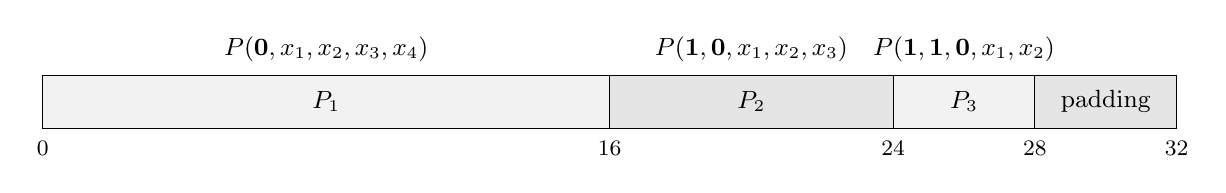
\begin{tikzpicture}[scale=0.45, every node/.style={font=\small}]
    \fill[gray!10] (0,0) rectangle (16,1.5);
    \fill[gray!20] (16,0) rectangle (24,1.5);
    \fill[gray!10] (24,0) rectangle (28,1.5);
    \fill[gray!20] (28,0) rectangle (32,1.5);

    \draw[black] (0,0) rectangle (32,1.5);
    \draw[black] (16,0) -- (16,1.5);
    \draw[black] (24,0) -- (24,1.5);
    \draw[black] (28,0) -- (28,1.5);

    \node at (8,0.75) {$P_1$};
    \node at (20,0.75) {$P_2$};
    \node at (26,0.75) {$P_3$};
    \node at (30,0.75) {padding};

    \node[below] at (0,-0.1) {\footnotesize 0};
    \node[below] at (16,-0.1) {\footnotesize 16};
    \node[below] at (24,-0.1) {\footnotesize 24};
    \node[below] at (28,-0.1) {\footnotesize 28};
    \node[below] at (32,-0.1) {\footnotesize 32};

    % Selector annotations above each section
    \node[above] at (8,1.6) {$P({\mathbf{0}}, x_1, x_2, x_3, x_4)$};
    \node[above] at (20,1.6) {$P({\mathbf{1}}, {\mathbf{0}}, x_1, x_2, x_3)$};
    \node[above] at (26,1.6) {$P({\mathbf{1}}, {\mathbf{1}}, {\mathbf{0}}, x_1, x_2)$};
\end{tikzpicture}
\caption{Simple stacking of $P_1, P_2, P_3$ into a single polynomial $P$}
\label{fig:stacking}
\end{figure}

Advantage of this approach: simplicity.

Drawback: padding overhead, i.e. it does not take advantage of the potential repetions at the end of each inner polynomial's evaluations.

\vspace{5mm}

There are alterntive ways to handle the stacking of multiple multilinear polynomials:

\begin{itemize}
    \item \textbf{Jagged PCS} \cite{jagged_pcs}: No padding overhead, at the cost of an additional sumcheck.
    \item  \textbf{Per-polynomial chunking}: decompose the non-repeated par of each inner polynomial into a small (think 3 or 4) number of power-of-two sized chunks, and concatenate all these chunks into a single large polynomial.
\end{itemize}

\textit{Note 3:} A meticulous implementation of WHIR could also take advantage of any potential repetitions in the committed polynomial, both at the FFT and the sumcheck level, leaving the Merklelisation as the main overhead.

\clearpage
\bibliographystyle{IEEEtran}
\bibliography{bibliography}

\end{document}